\section{Modelos de distribución de software SaaS}
\label{sec:modelos_negocio}

Hay una gran variedad de modelos de distribución de software, tal como pueden ser el modelo \textit{On-Premise}, el modelo \textit{Infrastructure as a Service} (IaaS) o el modelo \textit{Platform as a Service} (PaaS). Sin embargo, el modelo que más se utiliza en la actualidad es el modelo \textit{Software as a Service} (SaaS).

Años atrás, el software se distribuía principalmente a través de licencias perpetuas, donde los usuarios compraban una licencia para utilizar el software en sus propios servidores o computadoras. Este modelo requería que los usuarios gestionaran la infraestructura y el mantenimiento del software, lo que podía ser costoso y complicado. Esto significaba que el proveedor del software simplemente facilitaba el producto y el usuario debía hacerse cargo de la instalación, configuración y mantenimiento del mismo. Esto podía resultar complicado y costoso, especialmente para pequeñas y medianas empresas que no contaban con los recursos necesarios para gestionar su propia infraestructura. Esto es conocido como una infraestructura \textit{On-Premise}.

Con la llegada de internet y la nube, surgieron nuevos modelos de distribución de software que permitieron a las empresas ofrecer sus productos y servicios de manera más eficiente y escalable. El modelo SaaS es uno de los más populares y se basa en la idea de que el software se aloja en la nube y se accede a través de internet. Esto significa que los usuarios no necesitan instalar ni gestionar el software en sus propios servidores u ordenadores, sino que pueden acceder a él a través de un navegador web.

Sin embargo, la dependencia de la conexión a internet, la falta de control sobre la infraestructura y la seguridad de los datos son puntos críticos en el modelo. Además, los proveedores de SaaS suelen cobrar tarifas mensuales o anuales por el uso del software, pues el mantenimiento de la infraestructura y el soporte técnico son responsabilidad del proveedor.

Existen también otras alternativas, como pueden ser los modelos IaaS y PaaS. Cada uno de estos modelos tiene sus propias ventajas y desventajas, y dependiendo del tipo de negocio y las necesidades del cliente, uno puede ser más adecuado que otro. En la figura \ref{fig:modelos_negocio} se pueden observar los diferentes modelos de distribución de software y sus características.

\begin{figure}
    \centering
    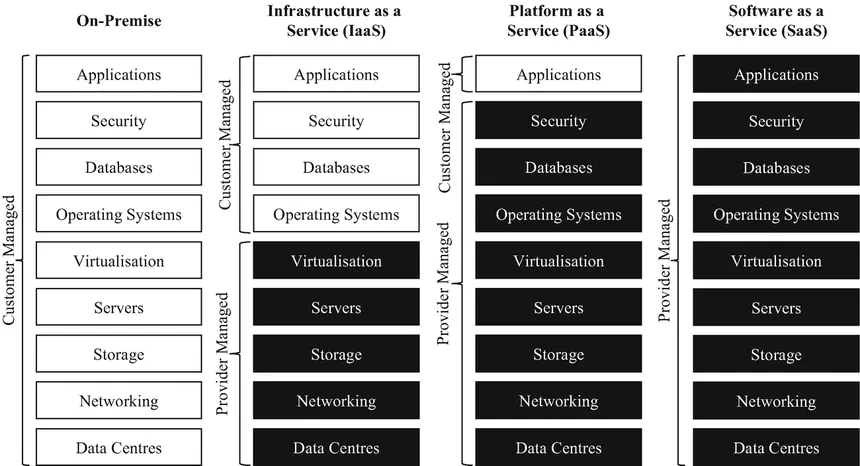
\includegraphics[width=0.8\textwidth]{figures/theoric_frame/comp_services.png}
    \caption{Modelos de distribución de software. Fuente: \cite{modelos_distirbucion}}
    \label{fig:modelos_negocio}
\end{figure}